%
%
% This is an example LaTeX file which uses the SANDreport class file.
% It shows how a SAND report should be formatted, what sections and
% elements it should contain, and how to use the SANDreport class.
%
% Get the latest version of the class file and more at
%    https://gitlab.sandia.gov/latex/sandreport-latex
%
\makeatletter
\def\input@path{{sand_report_template}}
\makeatother

\documentclass[report, 12pt]{SANDreport}

\usepackage{subcaption}
\usepackage{amsmath,bm}
\usepackage{tabularx}
\usepackage{multirow}
\usepackage{ragged2e}
\usepackage{enumerate}
\usepackage{hyperref}
\usepackage{listings}

\newcommand\YAMLcolonstyle{\color{red}\mdseries}
\newcommand\YAMLkeystyle{\color{black}\bfseries}
\newcommand\YAMLvaluestyle{\color{blue}\mdseries}

\makeatletter

% here is a macro expanding to the name of the language
% (handy if you decide to change it further down the road)
\newcommand\language@yaml{yaml}

\expandafter\expandafter\expandafter\lstdefinelanguage
\expandafter{\language@yaml}
{
  keywords={true,false,null,y,n},
  keywordstyle=\color{darkgray}\bfseries,
  basicstyle=\YAMLkeystyle,                                 % assuming a key comes first
  sensitive=false,
  comment=[l]{\#},
  morecomment=[s]{/*}{*/},
  commentstyle=\color{purple}\ttfamily,
  stringstyle=\YAMLvaluestyle\ttfamily,
  moredelim=[l][\color{orange}]{\&},
  moredelim=[l][\color{magenta}]{*},
  moredelim=**[il][\YAMLcolonstyle{:}\YAMLvaluestyle]{:},   % switch to value style at :
  morestring=[b]',
  morestring=[b]",
  literate =    {---}{{\ProcessThreeDashes}}3
                {>}{{\textcolor{red}\textgreater}}1     
                {|}{{\textcolor{red}\textbar}}1 
                {\ -\ }{{\mdseries\ -\ }}3,
}

% switch to key style at EOL
\lst@AddToHook{EveryLine}{\ifx\lst@language\language@yaml\YAMLkeystyle\fi}
\makeatother

\newcommand\ProcessThreeDashes{\llap{\color{cyan}\mdseries-{-}-}}

% \usepackage[table]{xcolor}

%\usepackage{draftwatermark}
%\SetWatermarkScale{.5}
%\SetWatermarkText{Sample, contains no OUO}

%if you want to use a clone of the SANDreport standard font, 
%  you must install `ebgaramond-maths` package (not included in
%  most standard LaTeX distributions
%\usepackage{ebgaramond} %includes old-style (hanging below the line) numbers.
%\usepackage[lining]{ebgaramond} %if you dont like old-style (hanging below the base line) numbers.
%\usepackage{ebgaramond-maths}

% Bonus: 
% Scientific Notation Command (built-in)
%  This command allows for a standard way to adding units and scientific notation
%    eliminating the need for the constant use of \mathrm and explicitely typing 10^n 
%    everytime you need a number in scientific notation 
%
%  The prototype command is:
%     \sci{mantissa}<exponent>[units]
%  Units will be typeset in mathrm so use standard notation (e.g. [g/cm^3])
%  other forms include:
%     * \sci{mantissa}<exponent>
%     * \sci{mantissa}[units]
%     * \sci{mantissa}

% ---------------------------------------------------------------------------- %
\newcommand{\stiff}{\operatorname{stiff}}
\newcommand{\realpart}{\operatorname{real}}
%\newcommand{\ats}{\operatorname{ats}}
\newcommand{\ats}{\operatorname{\ensuremath{\tau_a}}}
\newcommand{\vecbold}[1]{\boldsymbol{#1}}
\newcommand{\bx}{\vecbold{x}}
\newcommand{\avgstiff}{\alpha}
\newcommand{\avgstiffG}{\avgstiff_G}
\newcommand{\avgstiffS}{\avgstiff_\sigma}
\newcommand{\avgstiffF}{\avgstiff_F}
\newcommand{\avgL}{\alpha_{L^2}}
\newcommand{\preavgstiff}{\rm \operatorname{pre-avg~stiff}}
\newcommand{\preavgstiffG}{\preavgstiff_G}
\newcommand{\preavgstiffS}{\preavgstiff_\sigma}
\newcommand{\preavgstiffF}{\preavgstiff_F}
\newcommand{\bv}{\vecbold{v}}
\newcommand{\bu}{\vecbold{u}}
\newcommand{\RES}{\texttt{RES}}
\newcommand{\RESL}{\texttt{RES~L2}}
\newcommand{\RESstiff}{\texttt{RES~stiff}}
\newcommand{\by}{\bm{y}}
\newcommand{\bg}{\bm{g}}
\newcommand{\ba}{\bm{a}}
\newcommand{\bb}{\bm{b}}
\newcommand{\bc}{\bm{c}}
%\newcommand{\bv}{\bm{v}}
\newcommand{\bV}{\bm{V}}
\newcommand{\bnu}{\bm{\nu}}
\newcommand{\balpha}{\bm{\alpha}}
\newcommand{\bgamma}{\bm{\gamma}}
\newcommand{\bomega}{{\bm{\omega}}}
\newcommand{\btheta}{{\bm{\theta}}}
\newcommand{\bi}{\begin{itemize}}
\newcommand{\ei}{\end{itemize}}
\newcommand{\be}{\begin{equation}}
\newcommand{\ee}{\end{equation}}
\newcommand{\bea}{\begin{eqnarray}}
\newcommand{\eea}{\end{eqnarray}}
\newcommand{\bean}{\begin{eqnarray*}}
\newcommand{\eean}{\end{eqnarray*}}
\newcommand{\ben}{\begin{equation*}}        % eqn w/no number
\newcommand{\een}{\end{equation*}}
%\newcommand{\ben}{\[}
%\newcommand{\een}{\]}
\newcommand{\vtheta}{{\bm \theta}}
\newcommand{\vW}{{\bm W}}
\newcommand{\vb}{{\bm b}}
\newcommand{\valpha}{{\bm \alpha}}
\newcommand{\calD}{\mathcal{D}}
\newcommand{\R}{\mathbb{R}}
\newcommand{\E}{\mathbb{E}}

\newcommand{\bfu}{\mathbf{u}}
\newcommand{\bfp}{\mathbf{p}}
\newcommand{\bfc}{\mathbf{c}}
\newcommand{\bfy}{\mathbf{y}}
\newcommand{\bfb}{\mathbf{b}}
\newcommand{\bfK}{\mathbf{K}}
\newcommand{\bfW}{\mathbf{W}}
\newcommand{\bftheta}{\boldsymbol{\theta}}
\newcommand\vxi{{\bm \xi}}

% ==============================================================================
%                            Mike macros
% ==============================================================================

\definecolor{mjsb}{HTML}{00789A}
\definecolor{mjsg}{HTML}{2b8865}
\newcommand{\mjsnote}[1]{\textcolor{mjsb}{\texttt{\underline{mjs}:}} \textit{\textcolor{mjsg}{#1}}}
\newcommand{\eee}{E3SM}
\newcommand{\cpp}{C\nolinebreak\hspace{-.05em}\raisebox{.4ex}{\scriptsize\bf +}\nolinebreak\hspace{-.10em}\raisebox{.4ex}{\scriptsize\bf +}\ }
\newcommand{\und}{\textunderscore}
\newcommand{\dt}{\Delta t}
\newcommand{\gcell}{\cellcolor{gray!15}}
\newcommand{\dif}{\mathrm{d}}

% ==============================================================================

% ---------------------------------------------------------------------------- %
%
% Set the title, author, and date
%
  \title{TChem-atm: A performance portable toolkit for atmospheric chemistry mechanisms}

   

	\author{Oscar Diaz-Ibarra, Michael J. Schmidt, Cosmin Safta}
    \date{}


% ---------------------------------------------------------------------------- %
% Set some things we need for SAND reports. These are mandatory
%
\SANDnum{SAND2024-XXX}
\SANDprintDate{May 2024}

% ---------------------------------------------------------------------------- %
% The following definition does not have a default value and will not
% print anything, if not defined
%
\SANDsupersed{SAND1901-0001}{January 1901}


% ---------------------------------------------------------------------------- %
%
% Start the document
%
\begin{document}
    \maketitle
\justifying

    % ------------------------------------------------------------------------ %
    % An Abstract is required for SAND reports
    %
    \begin{abstract}
TChem-atm computes source terms and Jacobian matrices for chemical systems. It is a performance-portable software toolkit designed for complex kinetic mechanisms. We designed and implemented TChem-atm using Kokkos~\cite{kokkosweb,Carter:2014,Trott:2021:kokkos,Trott:2022:kokkos}

Software Design:
\begin{itemize}
  \item Modern C++.
  \item Kokkos programming model for performance portability.
  \item CMake build system.
  \item Numerical Jacobians and SACADO analytic Jacobians for all models.
  \item Coupling to external ODE solvers, e.g., Tines, Sundials (CVODE).
\end{itemize}

\begin{figure}[htp]
  \centering
  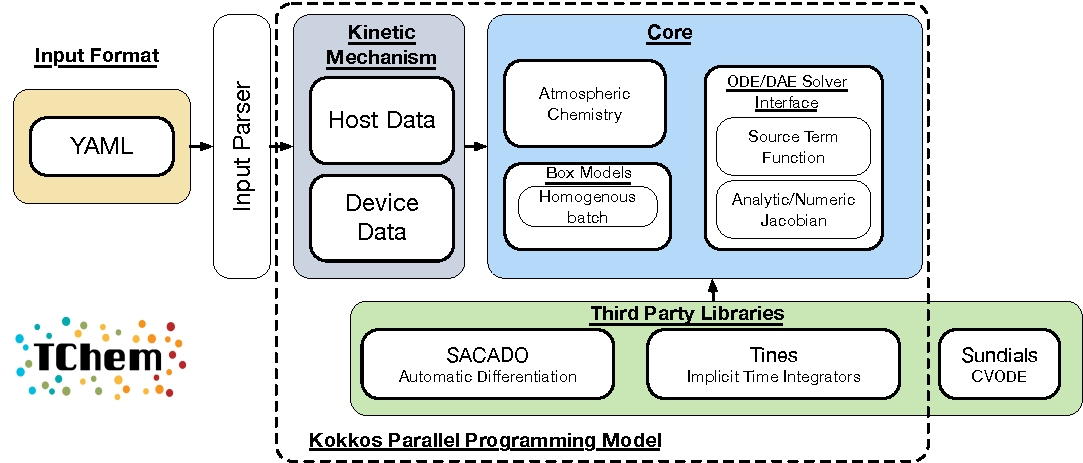
\includegraphics[width=1\textwidth]{../figures/TChem_atm.pdf}
  \caption{Ovierview of TChem-atm.}
\label{fig:method}
\end{figure}

As depicted in Figure~\ref{fig:method}, TChem-atm includes a parser for a YAML input file that constructs a kinetic model constant data object containing relevant parameters for the computation of the chemical source terms. It computes the reaction constants and rate of progress for all the reactions listed in the input files. Then, it calculates the net production rate or source terms for all species mentioned in the input files. TChem-atm automatically calculates the Jacobian matrix for the source terms using either finite differences (numerical Jacobian) or automatic differentiation (analytical Jacobian via SACADO). Furthermore, the computation of the source term and associated Jacobian is independent of the time integration solver in TChem-atm. Therefore, TChem-atm provides an interface for time integration (Box model) for the Tines and CVODE libraries. Finally, TChem-atm features a batched interface for evaluating the source term, Jacobian matrix, and time integration.

\end{abstract}


  %   % ------------------------------------------------------------------------ %
  %   % An Acknowledgement section is optional but important, if someone made
  %   % contributions or helped beyond the normal part of a work assignment.
  %   % Use \section* since we don't want it in the table of context
  %   %
   \cleardoublepage 
   \chapter*{Acknowledgement}
    \addcontentsline{toc}{chapter}{ACKNOWLEDGMENT}
  TChem-atm has been developed using the following funding sources:

\begin{itemize}

\item Sandia Laboratory Directed Research and Development (LDRD) projects "Bridging aerosol representations across scales with physics-constrained statistical learning" and "Benchmarking TChem for Potential Incorporation into E3SM as a Replacement Chemical Kinetics Solver."

\item The EAGLES project (https://climatemodeling.science.energy.gov/projects/enabling-aerosol-cloud-interactions-global-convection-permitting-scales-eagles), which was funded by
the Office of Science's Biological and Environmental
Research (https://science.osti.gov/ber) Program.

\item Exascale Catalytic Chemistry ECC Project; https://www.ecc-project.org/.

\end{itemize}


This work was supported by the Laboratory Directed Research and Development program at
Sandia National Laboratories, a multimission laboratory managed and operated by National
Technology and Engineering Solutions of Sandia LLC, a wholly owned subsidiary of Honeywell
International Inc. for the U.S. Department of Energy’s National Nuclear Security Administration
under contract DE-NA0003525.


  %  \cleardoublepage
  %   \section*{Acknowledgments}
	% TChem-atm has been developed using the following funding sources:

\begin{itemize}

\item Sandia Laboratory Directed Research and Development (LDRD) projects "Bridging aerosol representations across scales with physics-constrained statistical learning" and "Benchmarking TChem for Potential Incorporation into E3SM as a Replacement Chemical Kinetics Solver."

\item The EAGLES project (https://climatemodeling.science.energy.gov/projects/enabling-aerosol-cloud-interactions-global-convection-permitting-scales-eagles), which was funded by
the Office of Science's Biological and Environmental
Research (https://science.osti.gov/ber) Program.

\item Exascale Catalytic Chemistry ECC Project; https://www.ecc-project.org/.

\end{itemize}


This work was supported by the Laboratory Directed Research and Development program at
Sandia National Laboratories, a multimission laboratory managed and operated by National
Technology and Engineering Solutions of Sandia LLC, a wholly owned subsidiary of Honeywell
International Inc. for the U.S. Department of Energy’s National Nuclear Security Administration
under contract DE-NA0003525.

  %   \clearpage

    % ------------------------------------------------------------------------ %
    % The table of contents and list of figures and tables
    % Comment out \listoffigures and \listoftables if there are no
    % figures or tables. Make sure this starts on an odd numbered page
    %
    \cleardoublepage		% TOC needs to start on an odd page
    \tableofcontents
    \cleardoublepage
    \listoffigures
    \cleardoublepage
    \listoftables
    \cleardoublepage


  %   % ---------------------------------------------------------------------- %
  %   % An optional executive summary
  %   \clearpage
  %   \section*{Summary}
  %   \addcontentsline{toc}{section}{Summary}
	% \input{summary}


    % ---------------------------------------------------------------------- %
    % An optional glossary. We don't want it to be numbered
    % \clearpage
    % \section*{Nomenclature}
    % \addcontentsline{toc}{section}{Nomenclature}
    % \input{nomenclature}

    % ---------------------------------------------------------------------- %
    % This is where the body of the report begins; usually with an Introduction
    %
    \SANDmain		% Start the main part of the report

    % \ifthenelse{\boolean{reportSAND}}{
    %   \chapter{The First Chapter}
    % }{}

% \chapter{Overview}
% \label{ch:intro}

\chapter{Installation}
\label{ch:install}
TChem-atm requires the following third-party libraries:
\begin{itemize}
  \item Tines~\cite{tinesweb}
  \item Sacado~\cite{sacadoweb} 
  \item BLAS/LAPACK~\cite{openBLASweb, Wang:openBLAS:2013,Xianyi:openBLAS:2012}
  \item YAML-CPP~\cite{yaml}
  \item Sundials~\cite{SUNDIALS_gardner2022, SUNDIALS_hindmarsh2005}
  \item Gtest~\cite{gtestweb}
  \item Skywalker\cite{skywalkerweb}
\end{itemize}

These third-party libraries are submodules in TChem-atm. Thus, we can initialize them using the following command:

\begin{verbatim}
git submodule update --init --recursive
\end{verbatim}

\section{Obtaning TChem-atm}

TChem-atm is open-source code available on GitHub (https://github.com/sandialabs/tchem-atm)~\cite{tchem-atm}.

\section{Building and installing third-party libraries}

The script \verb|scripts/tpls_bld.sh| clones, builds, and installs TChem-atm's third-party libraries. To use this script, one must provide compiler information as follows:

\begin{verbatim}
MY_CC=gcc # C++ compiler
MY_CXX=g++ # C++ compiler
MY_FC=gfortran # Fortran compiler
\end{verbatim}

To build/install with CUDA \verb|ON| or \verb|OFF|, use:

\begin{verbatim}
CUDA="ON" # Set to ON/OFF to compile TChem-atm with or without NVIDIA-GPUs support.
\end{verbatim}

Additionally, specify the root directory for installing/building the third-party libraries:

\verb|ROOT=/path/to/tchem-atm/|.

These variables are located in the top section of the \verb|scripts/tpls_bld.sh| script.

This script initializes the submodules and installs/builds the third-party libraries in the \verb|ROOT/HOST| or \verb|ROOT/DEVICE| directory, depending on whether \verb|CUDA=OFF| or \verb|CUDA=ON|. Since Kokkos can be installed/built with both CUDA \verb|ON| and \verb|OFF|, this script installs it in both \verb|ROOT/HOST| and \verb|ROOT/DEVICE|, while the other libraries are installed in \verb|ROOT/HOST|. Therefore, one must run this script using \verb|CUDA=OFF| to install all third-party libraries and run it a second time with \verb|CUDA=ON| if an NVIDIA GPU is available.

\section{Building and installing TChem-atm and Tines}

The script \verb|scripts/build_script.sh| builds and installs TChem-atm and Tines. Similar to the script for third-party libraries, in \verb|scripts/build_script.sh|, one must provide the compiler information:

\begin{verbatim}
MY_CC=gcc # C++ compiler
MY_CXX=g++ # C++ compiler
MY_FC=gfortran # Fortran compiler
\end{verbatim}

To build/install with CUDA ON (or OFF), use:

\verb|CUDA="ON" # Set to ON/OFF to compile TChem with NVIDIA-GPUs|

In addition, this script adds the option to turn \verb|SACADO="ON"| or \verb|SACADO="OFF"| for enabling or disabling automatic differentiation using the SACADO library.

The installation path for the third-party libraries is specified by \verb|INSTALL_BASE_HOST|, and \verb|ROOT=/path/to/tchem-atm| is where TChem-atm and Tines are installed. If CUDA is \verb|ON|, libraries will be installed in the \verb|ROOT/DEVICE| directory. Otherwise, they will be installed in the \verb|ROOT/HOST| directory.

\chapter{Theoretical Background}
\label{ch:theo}
TChem-atm computes the source term or the right-hand side of the $k$ gas-species equation:

\begin{equation}\label{eq:ode_vmr}
  \frac{\dif{} \eta_k}{\dif{} t}=\dot{\omega}_k,
\end{equation}

and its associated Jacobian matrix, $\textbf{J}_{ij} = \frac{\partial \dot{\omega}_i}{\partial \eta_j }$, which is evaluated using either finite differences or automatic differentiation via the Tines library or the Sacado library. Furthermore, TChem-atm has an interface for Tines or CVODE (ODE(ordinary differential equations) solver) to advance in time the volumetric mixing ratio (vmr, $\eta_k$ ) of gas species, $k$.

The net production rate of species $k$, $\dot{\omega}_k$, or the right-hand side of the previous equation is computed using:

\begin{equation}\label{eq:net_production_rates}
  \dot{\omega}_k=\sum_{i=1}^{N_{\text{react}}}\nu_{ki}q_i,\quad \nu_{ki}=\nu''_{ki}-\nu'_{ki},
\end{equation}

where $q_i$ is the rate of progress of reaction $i$, $N_{\text{react}}$ is the number of reactions, and $\nu''_{ki}$/$\nu'_{ki}$ are the stoichiometric coefficients of species $k$ in reaction $i$ for the reactant/product sides of the reaction, respectively. The rate of progress of reaction $i$, $q_i$, is computed as

\begin{equation}\label{eq:rate_of_progress}
  q_i={k_f}_i\prod_{j=1}^{N_{\text{spec}}}\eta_j^{\nu'_{ji}},
\end{equation}

where $N_{\text{spec}}$ is the number of species, ${k_f}_i$ is the reaction constant of reaction $i$. The reaction constant ${k_f}_i$ can take several functional forms depending on the reaction type. We present below the reaction types that are available in TChem-atm.


\section{Reaction types}
Currently, TChem-atm can reproduce gas chemistry for two complex reaction mechanisms: the gas chemistry of $\eee{}$ v3, i.e., the UCI chemistry (University of California Irvine), and the Carbon Bond 2005 chemical mechanism, which is well-formulated for urban to remote troposphere conditions~\cite{Yarwood2005,Dawson2022}.
To represent these mechanisms, TChem-atm implements Troe, Arrhenius, Troe-Arrenious ratio, and Custom-H2O2 reaction types.

Next, we present the expression for the forward rate constant of the reaction types implemented in TChem-atm. In these equations, $\mathrm{T}$, $\mathrm{P}$, $[M]$ correspond to the temperature, pressure, and air concentration.

\subsection{Arrhenius type}

The Arrhenius type (\verb|type: ARRHENIUS|) is computed by

\begin{equation}
k_f = A \mathrm{exp} \Big( \frac{C}{\mathrm{T}} \Big)  \frac{\mathrm{T}}{D}^B (1+ E\,\mathrm{P})
\end{equation}

Where, $A$, $B$, $C$, and $D$ are kinetic constants. As an example, the following reaction from the Carbon Bond 5 mechanism,

\begin{equation}
O_3 + NO \rightarrow NO_2 + O_2,
\end{equation}

has the following information provided using the following YAML configuration:

\begin{lstlisting}[language=yaml]
- MUSICA_name: R3
  reactants:
    O3: 1
    NO: 1
  products:
    NO2: 1
  type: ARRHENIUS
  coefficients:
    A: 3e-12
    B: 0.0
    C: -1500.0
    D: 0.0
\end{lstlisting}

Under the `reactants`/`products`, the name and stoichiometric coefficient ($\nu''_{ki}$ /$\nu'_{ki}$) of each species is listed.

Note that in the previous reaction, $O_2$ is not considered a product in the computation of $k_f$.

\subsection{Troe type}
The Troe type (\verb|type: TROE|) is computed by

\begin{equation}
k_f=\frac{k_0[M]}{1+\frac{k_0[M]}{k_{\infty}}}F_c^{\left(1+\left(\frac{log_{10} \big(\frac{k_0[M]}{k_{\infty}} \big)}{N}\right)^2 \right)^{-1}},
\end{equation}

where, the $k_0$ and $k_{\infty}$ are computed with the following Arrhenius expresion.

\begin{equation}
k_0 = k_{0_A} \mathrm{exp} \Big( \frac{k_{0_C}}{\mathrm{T}} \Big)  \left(\frac{\mathrm{T}}{300}\right)^{k_{0_B}}
\end{equation}

\begin{equation}
k_{\infty} = k_{\infty_A} \mathrm{exp} \Big( \frac{k_{\infty_C}}{\mathrm{T}} \Big) \left(\frac{\mathrm{T}}{300}\right)^{k_{\infty_B}}
\end{equation}

As an example of one reaction from the carbon bond 5 mechanism,

\begin{equation}
O + NO_2 \rightarrow NO_3
\end{equation}

The kinetic constants are passed using the following format:

\begin{lstlisting}[language=yaml]
- MUSICA_name: R5
  reactants:
    O: 1
    NO2: 1
  products:
    NO3: 1
  type: TROE
  coefficients:
    k0_A: 2.5e-31
    k0_B: -1.8
    k0_C: -0.0
    kinf_A: 2.2e-11
    kinf_B: -0.7
    kinf_C: -0.0
    Fc: 0.6
    N: 1.0
\end{lstlisting}

We use a modified version of the Troe reaction for the UCI mechanism using the \verb|type : JPL|.

For example, for the \verb|uci6| reaction in the UCI mechanism:

\begin{equation}
HNO_3 + OH \rightarrow NO_3 + H_2O
\end{equation}

\begin{lstlisting}[language=yaml]
- coefficients:
    k0_A: 6.5e-34
    k0_B: 0
    k0_C: 1335
    Fc: 1
    kinf_A: 2.7e-17
    kinf_B: 0
    kinf_C: 2199
  type: JPL
  note: uci6
  adjust_reaction:
  - M
  id: '52'
  reactants:
    HNO3: 1
    OH: 1
  products:
    NO3: 1
    H2O: 1
\end{lstlisting}
Note that in the \verb|JPL| type \verb|N=1|.

\subsection{Custom H2O2 type}

The rate constant for the custom H2O2 type (\verb|type: CMAQ_H2O2|) can not be expressed as the combination of Arriheous and Troe reaction types. Hence, TChem-atm has a specific type of reaction for this reaction.

\begin{equation}
k_f = A_1 \mathrm{exp} \Big( \frac{C_1}{\mathrm{T}} \Big)
\left(\frac{\mathrm{T}}{300}\right)^{B_1} + A_2 \mathrm{exp} \Big ( \frac{C_2}{\mathrm{T}} \Big) \left(\frac{\mathrm{T}}{300}\right)^{B_2} \mathrm{conv}
\end{equation}

where, $\mathrm{conv} = \frac{N_A}{R \times 10^{-12}} \frac{P}{T}$ and $N_A=6.02214179 \times 10^{23}$ is Avogadro's number ($\mathrm{mole}^{-1}$) and $R=8.314472$ is the universal gas constant ($J \mathrm{mole}^{-1}K^{-1}$).

As an example of this reaction from the carbon bond 5 mechanism:

\begin{equation}
2HO_2 \rightarrow H_2O_2
\end{equation}

\begin{lstlisting}[language=yaml]
- MUSICA_name: R34
  reactants:
    HO2: 2
  products:
    H2O2: 1
    DUMMY: 1
  type: CMAQ_H2O2
  coefficients:
    k1_A: 2.3e-13
    k1_C: 600.0
    k2_A: 1.7e-33
    k2_C: 1000.0
\end{lstlisting}
\subsection{Custom OH\_HNO3}

The carbon bond 5 mechanism employs this reaction type and can be expressed as the sum of Arrhenius and Troe reaction types, i.e., $k_f=k_{troe} + k_{arrhenius}$. Hence, one must specify two reactions in the YAML input files. For example:

\begin{equation}
HNO_3 + OH \rightarrow NO_3
\end{equation}

\begin{lstlisting}[language=yaml]
- coefficients:
    A: 2.4e-14
    C: 460.0
  note: CMAQ_OH_HNO3
  products:
    NO3: 1.0
  reactants:
    HNO3: 1.0
    OH: 1.0
  type: ARRHENIUS
- coefficients:
    k0_A: 6.5e-34
    k0_C: 1335.0
    kinf_A: 2.7e-17
    kinf_C: 2199.0
    Fc : 1
  note: CMAQ_OH_HNO3
  products:
    NO3: 1.0
  reactants:
    HNO3: 1.0
    OH: 1.0
  type: TROE
\end{lstlisting}

\subsection{Troe-Arrhenius ratio Type}

This reaction type (\verb|type: R_JPL_ARRHENIUS|) is computed as the ratio between Troe (or JPL) and Arrhenius types, i.e., $k_f=k_{troe}/k_{arrhenius}$.

The addition of this reaction type to represent UCI reactions required custom-defined rate coefficients (UCI \#7-9). As an example, for FIXME%[`uci7`](https://github.com/E3SM-Project/scream/blob/a73d48a5f8556e5240b64b037bc60d42cb5f2413/components/eam/src/chemistry/mozart/llnl_O1D_to_2OH_adj.F90#L184) reaction:

\begin{equation}
HO_2NO_2 + M \rightarrow HO_2 + NO_2 + M
\end{equation}

\begin{lstlisting}[language=yaml]
- coefficients:
    k0_A: 1.9e-31
    k0_B: -3.4
    Fc: 0.6
    kinf_A: 4e-12
    kinf_B: -0.3
    A: 2.1e-27
    B: 0
    C: 10900.0
  type: R_JPL_ARRHENIUS
  note: uci7
  adjust_reaction:
  - M
  id: '57'
  reactants:
    HO2NO2: 1
    M: 1
  products:
    HO2: 1
    NO2: 1
    M: 1
\end{lstlisting}
\subsection{usr\_DMS\_OH}

The reaction type \verb|usr_DMS_OH| is part of the UCI mechanism and is hard-coded in the [\verb|mo_usrrxt|]FIMXE
%(https://github.com/E3SM-Project/scream/blob/a73d48a5f8556e5240b64b037bc60d42cb5f2413/components/eam/src/chemistry/mozart/mo_usrrxt.F90#L683) 
submodule in $\eee$'s code. In TChem, we reformulate this reaction type as a Troe (or JPL) reaction type using the following configuration.

\begin{lstlisting}[language=yaml]
- coefficients:
    k0_A: 3.57e-43
    k0_B: 0
    k0_C: 7810
    Fc: 1
    kinf_A: 3.0909090909090913e-12
    kinf_B: 0
    kinf_C: 350
  type: JPL
  note: usr_DMS_OH
  adjust_reaction: [M, M]
  id: '89'
  reactants:
    DMS: 1
    OH: 1
  products:
    SO2: 0.5
    HO2: 0.5
\end{lstlisting}

\subsection{usr\_SO2\_OH}

The reaction type \verb|usr_SO2_OH| is part of the UCI mechanism and is hard-coded in the [\verb|mo_usrrxt|]
FIXME%(https://github.com/E3SM-Project/scream/blob/a73d48a5f8556e5240b64b037bc60d42cb5f2413/components/eam/src/chemistry/mozart/mo_usrrxt.F90#L693) 
submodule in $\eee$'s code. In TChem, we reformulate this reaction type as a Troe (or JPL) reaction type using the following configuration.

\begin{lstlisting}[language=yaml]
- coefficients:
    k0_A: 3e-31
    k0_B: -3.3
    k0_C: 0
    Fc: 0.6
    N: 1.0
    kinf_A: 1.5e-12
    kinf_B: 0
    kinf_C: 0
  type: JPL
  note: usr_SO2_OH
  adjust_reaction: [M, M]
  id: '90'
  reactants:
    SO2: 1
    OH: 1
  products:
    H2SO4: 1
\end{lstlisting}

\subsection{Modifier prod O1D}

Reaction types [UCI 1, 2, 3]
%(https://github.com/E3SM-Project/scream/blob/a73d48a5f8556e5240b64b037bc60d42cb5f2413/components/eam/src/chemistry/mozart/llnl_O1D_to_2OH_adj.F90#L152) 
in the UCI mechanism require a modifier to compute the reaction rate. We did not include this modifier under the \verb|reaction| section of the input file; instead, we created the section \verb|modifier_prod_O1D|.

\begin{equation}
\mathrm{factor} = \frac{\mathrm{prod_{O1D}}}{fc}
\end{equation}

where, $fc$

\begin{equation}
fc = A1\, \mathrm{exp} \Big(\frac{C1}{\mathrm{T}} \Big) * [\mathrm{N_2}] +
A2\, \mathrm{exp} \Big(\frac{C2}{\mathrm{T}} \Big) * [\mathrm{O_2}] +
A3\, \mathrm{exp} \Big(\frac{C3}{\mathrm{T}} \Big) * [\mathrm{H_2O}]
\end{equation}

The YAML configuration for this modifier is :

\begin{lstlisting}[language=yaml]
modifier_prod_O1D:
  coefficients:
    A1: 2.15e-11
    C1: 110.0
    A2: 3.3e-11
    C2: 55.0
    A3: 1.63e-10
    C3: 60.0
  species_name_1: N2
  species_name_2: O2
  species_name_3: H2O
  reaction_list:
  - 22
  - 23
  - 24
  photolysis_reaction_index: 0
\end{lstlisting}
Here, under \verb|coefficients|, the kinetic parameters are presented. The species involved in this factor are listed with \verb|`species_name_1`| to \verb|`species_name_2`|. Note that TChem will find the index of this species. The \verb|reaction_list| presents the index of reaction, where this modifier is applied. Finally, \verb|photolysis_reaction_index| is the index of the $\mathrm{prod_{O1D}}$ reaction.

Future work will convert \verb|reaction_list| from a list of indexes to reaction IDs. Thus, one does not need to know the index of each reaction before running a TChem simulation. Furthermore, \verb|photolysis_reaction_index| will be converted from index to reaction ID.

\chapter{Input file}

\subsection{Gas chemistry input file}

The YAML input file for atmospheric chemistry consists of five sections:

\begin{itemize}
\item \verb|environmental_conditions|: pressure and temperature of individual cells.
\item \verb|initial_state|: initial species concentration within the cells.
\item \verb|reactions|: list of reactions with rate parameters and reaction type.
\item \verb|constant_species|: species that are part of the reaction mechanism but are assumed constant.
e.g., invariant species.
\item \verb|species|: list of species names.
\end{itemize}

For example, for the toy reaction $A \rightarrow B$, simulation with N cells, one reaction, and three species


\begin{lstlisting}[language=yaml]
NCAR-version: v1.0
environmental_conditions:
  pressure:
    evolving: false
    initial_value: [P1, ..., PN]
    units: Pa
  temperature:
    evolving: false
    initial_value: [T1, ..., TN]
    units: K
initial_state:
  A:
    initial_value: [A1, .., AN]
    units: mol m-3
  M:
    initial_value: [M1, .., MN]
    units: mol m-3
reactions:
- coefficients:
  products:
    B: 1.0
  reactants:
    A: 1.0
  type: ARRHENIUS
constant_species:
- description: tracer-CONSTANT
  name: M
species:
- description: A
  name: A
- description: B
  name: B
\end{lstlisting}

A description of the reaction types currently implemented in TChem-atm is presented in theoretical background section~\ref{ch:theo}. In addition, a set of examples of input files is presented under \verb|/src/examples/runs/atmopheric_chemistry|.

\chapter{Examples}
\section{Carbon Bond 5}

We adapted the Carbon Bound 5 reaction mechanism from the FIXME
%[CAMP chemistry code](https://github.com/open-atmos/camp/tree/main/mechanisms/cb05cl_ae5).

Mechanism details:

\begin{itemize}
\item Number of Species: 67
\item Number of Reactions: 187
\item Arrhenius type reactions: 168
\item CMAQ\_H2O2 type reactions : 3
\item Troe type reactions: 16
\item Sources e.g., EMISSION: 14
\end{itemize}

The mechanism in the CAMP solver has 26 photolysis reactions, which we replace with Arrhenius-type reactions with energy = 0  and temperature coefficient = 1.

Scripts to run and plot the outputs of this example are at: \verb|src/examples/runs/atmospheric_chemistry/CB05CL_AE5|. The bash script to run this mechanism is shown below:


\begin{verbatim}
exec=$TCHEM_INSTALL_PATH/examples/TChem_AtmosphericChemistry.x

run_this="$exec --chemfile=config_full_gas.yaml \
          --outputfile=full_gas.dat \
          --time-iterations-per-interval=10 \
          --tol-time=1e-10 \
          --dtmin=1e-20 \
          --dtmax=10 \
          --tend=600\
          --atol-newton=1e-18 \
          --rtol-newton=1e-8 \
          --max-newton-iterations=20 \
          --max-time-iterations=20000"

echo $run_this
eval $run_this
\end{verbatim}

Here, the \verb|TChem_AtmosphericChemistry.x| executable is a box model that integrates in time a list of species using the mechanism file from input \verb|chemfile|, which in this case is the \verb|config_full_gas.yaml|. The box model only considers chemical reactions. The executable saves the time profiles for the species in \verb|outputfile=full_gas.dat|. In the example directory, the jupyter-notebook \verb|PlotFullGas| plots the time profiles of each species from the TChem-atm and CAMP outputs. Note that the CAMP output was previously computed and saved in the TChem-atm repository.

The \verb|TChem_AtmosphericChemistry.x| executable allows to change time integration parameters of the 
FIXME 
% [TrBDF2 solver](https://github.com/sandialabs/Tines?tab=readme-ov-file#timeintegration).
 First, the Newton solver parameters are the
absolute (\verb|atol-newton|), relative tolerance (\verb|rtol-newton|), and the maximum number of iterations (\verb|max-newton-iterations|). Second, the time step size is controlled using the \verb|tol-time| parameter and the maximum (\verb|dtmax|) and minimum (\verb|dtmin|) time step values. Third, the parameters either \verb|tend| or \verb|max-time-iterations| will end the simulation. Finally, one can get additional help information from the \verb|TChem_AtmosphericChemistry.x| executable using \verb|TChem_AtmosphericChemistry.x --help|.


FIXME
%![TChem-atm vs CAMP](figures/carbonB5TChemvsCAMP.png)
Comparing TChem-atm and CAMP outputs using the Carbon Bound 5 mechanism.

\section{UCI-E3SM version 3 chemistry}

E3SM version 3 uses the UCI mechanism to model gas chemistry using separate reaction mechanisms for the Troposphere and Stratosphere. As part of the Sandia LDRD project "Benchmarking TChem for Potential Incorporation into E3SM as a Replacement Chemical Kinetics Solver"[CITE], we created TChem-atm input files for the UCI mechanism. In addition, we implemented reaction types that are needed to reproduce this chemistry mechanism in TChem-atm.

E3SM employs the Community Atmospheric Model Pre-Processor (CAMPP) to generate a set of Fortran files to represent and solve the chemical kinetic model, which includes reaction coefficients, the hand side of volumetric mixing ratio (vmr, denoted $\eta$), and ODE solvers (Implicit/Explicit solver). Ultimately, CAMPP aims to compute an updated vmr ($\eta_{t+\Delta t}$) for the troposphere and stratosphere.

For additional information on this LDRD project, we recommend to read the [SAND2024-01807R report]
% (/../sand_report/QTI_tchemV1.pdf)
[CITE]. As described in the SAND2024-01807R report, we employed TChem-atm to time advance one-time step and compare these outputs with E3SM output in six different locations; see table below. We compute the relative root mean square error (RRMSE) of the difference between the E3SM and TChem-atm outputs. Using this approach, we verified the input files and implementation of TChem-atm.


\begin{table}[htbp]
    \centering
    \begin{tabular}{|c|c|c|c|}
        \hline
        Abbreviation & Latitude & Longitude & Location \\
        \hline
        LA & 34.0549 & -118.2426 & Los Angeles, CA, USA \\
        BRW & 71.323 & -156.6114 & North Slope, AK, USA \\
        MHD & 53.326 & -9.899 & Halfmace, County Galway, Ireland \\
        PSA & -64.7742 & -64.0527 & Palmer Station, Antarctica \\
        RPB & 13.165 & -59.432 & Ragged Point, Barbados \\
        SYO & -69.0125 & 39.59 & Showa Station, Antarctica \\
        ZEP & 78.9067 & 11.8883 & Zeppelin mountain, Ny-\AA lesund, Norway \\
        \hline
    \end{tabular}
    \caption{Location Information}
    \label{tab:location-info}
\end{table}


\subsection{Troposphere mechanism}

The bash scripts and input files for the UCI chemistry in the troposphere are located at \verb|src/examples/runs/uci_col|. In this directory, we split the input file of TChem-atm into two input files. One has initial conditions, and the other file lists reactions, constant species, and active species. The chemistry file of the UCI mechanism is located at \verb|src/examples/runs/uci_col/uci_v2_test3.yaml|. The initial conditions file for one of the UCI tests is located at \verb|src/examples/runs/uci_col/input_conditions_col.yaml|, corresponding to a set of cells for one location in an E3SM simulation.

Mechanism details:

\begin{itemize}
    \item Number of species: 82
    \item Number of invariants or constant species: 29
    \item Number of reactions: 106
    \item Number of Arrhenius-type reactions: 71
    \item Number of JPL-Troe type reactions: 10
    \item Number of Ratio JPL-Arrhenius type reactions: 3
    \item Number of Photolysis rates: 22
\end{itemize}


A run script for the UCI mechanism is presented next:

\begin{verbatim}
exec=\$TCHEM_INSTALL_PATH/examples/TChem_AtmosphericChemistryE3SM.implicit_euler.x
input=\$TCHEM_INSTALL_PATH/examples/runs/atmospheric_chemistry/uci_col/uci_v2_test3.yaml
inputFile=\$TCHEM_INSTALL_PATH/examples/runs/atmospheric_chemistry/uci_col/input_conditions_multi_col.yaml
run_this="\$exec --chemfile=\$input \\
          --inputfile=\$inputFile \\
          --outputfile=full_gas.dat \\
          --time-iterations-per-interval=100 \\
          --tol-time=1e-6 \\
          --dtmin=1800 \\
          --dtmax=1800 \\
          --tend=1800 \\
          --atol-newton=1e-18 \\
          --rtol-newton=1e-8 \\
          --max-newton-iterations=20 \\
          --max-time-iterations=20000"

echo \$run_this
eval \$run_this
\end{verbatim}


Here, TChem-atm is using an implicit euler solver. The \verb|inputfile| flag allows to pass the initial condition files as an independent file of the \verb|chemfile|. Furthermore, TChem-atm also offers executables for Tines-TrBDF2 solver, \verb|TChem_AtmosphericChemistryE3SM.x| and for CVODE, \verb|TChem_AtmosphericChemistryE3SM_CVODE.x|; Note the CVODE-TChem-atm executable works only in CPUs.

FIXME
%![E3SM vs TChem-atm Troposhere](figures/net_production_rate_worst.png)
Parity plot for rate of progress in the troposphere. E3SM outputs are produced by CAMPP’s generated code. There are 104 reactions, and we only display the 10 with the larges RRMSE for the locations given in previous table. RRMSE per location is presented in each plot. The net production rates correspond to the RHS of the equations solved by E3SM and TChem.


\subsection{Stratosphere mechanism}

The chemistry file of the UCI mechanism of the stratosphere is located at \verb|src/examples/runs/uci_col/uci_explicit_mech.yaml|. The initial conditions file for one of the UCI tests is located at \verb|src/examples/runs/uci_col/input_conditions_explicit_part_multi_col.yaml|, which corresponds to one set of cells for one location in an E3SM simulation.

Mechanism details:

\begin{itemize}
    \item Number of species: 7
    \item Number of invariants or constant species invariants: 3
    \item Number of reactions: 5
    \item Number of Arrhenius-type reactions: 3
    \item Number of JPL-Troe type reactions: 2
\end{itemize}

E3SM uses an explicit Euler solver to time integrate gas chemistry in the Stratoshere. In TChem-atm, we also implemented an explicit Euler solver.


\begin{verbatim}
exec=$TCHEM_INSTALL_PATH/examples/TChem_AtmosphericChemistryE3SM.explicit_euler.x
input=$TCHEM_INSTALL_PATH/examples/runs/atmospheric_chemistry/uci_col/uci_explicit_mech.yaml
inputFile=$TCHEM_INSTALL_PATH/examples/runs/atmospheric_chemistry/uci_col/input_conditions_explicit_part_multi_col.yaml
run_this="$exec --chemfile=$input \
          --inputfile=$inputFile \
          --outputfile=full_gas_stratosphere.dat \
          --time-iterations-per-interval=100 \
          --tol-time=1e-6 \
          --dtmin=1800 \
          --dtmax=1800 \
          --tend=1800 \
          --atol-newton=1e-18 \
          --rtol-newton=1e-8 \
          --max-newton-iterations=20 \
          --max-time-iterations=20000"

echo $run_this
eval $run_this
\end{verbatim}


FIXME
% [E3SM vs TChem-atm Stratoshere](figures/net_production_rates_stratosphere.png)

Parity plot of net production rates(RHS) in the stratosphere. RRMSE per location is presented in each plot. The net production rates correspond to the RHS of the equations solved by E3SM and TChem.



% \cleardoublepage
% \chapter{DETAILED DESCRIPTION OF RESEARCH AND DEVELOPMENT AND METHODOLOGY}
%   \input{methodology}

% \chapter{RESULTS AND DISCUSSION}
%   \input{results}
% %
% \cleardoublepage
% \chapter{ANTICIPATED OUTCOMES AND IMPACTS}
%  \input{outcomes}
% \cleardoublepage
% \chapter{CONCLUSION}
%   \input{conclusion}

% \cleardoublepage


    % ---------------------------------------------------------------------- %
    % References
    %
    % Comment \nocite{*} to not cite every reference in your master library, 
    % just the ones cited in this document. 
    \nocite{*}

    \clearpage

    % If not, we need to define it.
    \providecommand*{\phantomsection}{}
    \phantomsection
    % \ifthenelse{\boolean{reportSAND}}{
    %   \addcontentsline{toc}{chapter}{References}
    % }{
    %   \addcontentsline{toc}{section}{References}
    % }
    %\small
    \bibliographystyle{abbrv}
    \bibliography{ref}


    % ------------------------,---------------------------------------------- %
  %   %
  %   \appendix
  %     \chapter{Looking Backward}

  %   \section{Historical Perspective}
	% \input{CommonHistory}


  %   \chapter{Some Other Appendix}
	% \input{CommonAppendix}

        
    % \printindex
    
    %
% This is an example of how to create the distribution page. Some
% distributions are required by Sandia; e.g. the housekeeping copies.
% Depending on the type of report; e.g. CRADA, Patent Caution, etc.
% additional distribution lines may have to be added. See the
% "Guide for Preparing SAND Reports"
%
% SANDdistribution takes CA or NM as an optional argument. If given,
% the approrpiate housekeeping copies are inserted autmatically.
% Inside the SANDdistribution environment, several commands can be used
% insert the distributions for CRADA, LDRD, etc. See example below.
%
% You can leave the CA or NM option off and not use any of the SANDdist*
% commands. This will allow you to create a distribution list manually.
%
\begin{SANDdistribution}[NM]
\addcontentsline{toc}{chapter}{DISTRIBUTION}
    % Housekeeping copies necessary for every unclassified report:
    % \SANDdistCRADA	% If this report is about CRADA work
    % \SANDdistPatent	% If this report has a Patent Caution or Patent Interest
    \SANDdistLDRD	% If this report is about LDRD work


    \SANDdistInternalEmail{Amanda Barry}{01901}{anbarry@sandia.gov}
    \SANDdistInternalEmail{Andrew Salinger}{01446}{agsalin@sandia.gov}

    % % Some external Addresses
    % \SANDdistExternal{1}{A Name}{An Address \newline 99 $99^{\texttt{th}}$ street NW \newline City, State}
    % \SANDdistExternal{3}{Name One \newline Name Two \newline Name Three}{Some Address\newline and street \newline City, State}
    % \bigskip

    % % Example of external email address
    % \SANDdistExternalEmail{John Deer}{john.deer@lawnmowersrus.com}{Lawnmowers R US}

    % % The following MUST BE between the external and internal distributions!
    % % \SANDdistClassified % If this report is classified


    % % Internal Addresses
    % \SANDdistInternal{1}{1319}{Rolf Riesen}{1423}
    % \SANDdistInternal{1}{1110}{Another One}{01400}

    % % Example of a mail channel use (instead of a mail stop)
    % \SANDdistInternalM{1}{M9999}{Someone}{01234}
    
    % % Example of internal email address
    % \SANDdistInternalEmail{John Doe}{1554}{jdoe@sandia.gov}

\end{SANDdistribution}

    

\end{document}
